\section{Numerical experiments}
\label{sec:results}

This section evaluates three properties of the pipeline: conservativeness,
accuracy relative to the exact roots of the dataset, and cost on each processor.
\Cref{sec:results:cons,sec:results:ref} address the first two. The remainder of
the section reports cost, including the configurations on which the pipeline is
the slower of the two.

\subsection{Experimental setup}
\label{sec:results:setup}

All measurements are taken on the CSCS Alps system, on nodes built from the
\textsc{NVIDIA GH200} Grace Hopper superchip~\citep{nvidia2023gh200}. A node
carries four modules, each pairing a Grace host with a Hopper device over a
cache-coherent NVLink-C2C link, and every measurement here uses a \emph{single}
module, its $72$ Grace cores and its one Hopper in the same allocation, so that
a host and a device number quoted together describe one module and not a node.
Host threads are bound to that module with \texttt{numactl}, since an unbound
run spreads across all four. \Cref{tab:hardware} states the two processors.

\begin{table}[htbp]
  \centering
  \caption{The two processors of one \textsc{GH200} module, as reported by the
    operating system and the CUDA device properties on the compute nodes used.
    Peak \textsc{fp64} is derived from those clocks and the per-unit counts of
    the two architectures~\citep{arm2022neoversev2,nvidia2022hopper}; the
    bandwidth row is the best of ten \textsc{stream} triad passes.}
  \label{tab:hardware}
  \fittable{%
  \begin{tabular}{lll}
    \toprule
     & Grace (host) & Hopper (device) \\
    \midrule
    architecture & Arm Neoverse V2 & NVIDIA Hopper, sm\_90 \\
    parallel units & $72$ cores & $132$ multiprocessors \\
    maximum clock & $3.42$ GHz & $1.98$ GHz \\
    vector width & $128$-bit SVE2 & $32$-thread warp \\
    threads in flight & $72$ & $270{,}336$ \\
    L1 / shared memory & $64$ KiB per core & $228$ KiB per multiprocessor \\
    L2 cache & $1$ MiB per core & $60$ MiB \\
    L3 cache & $114$ MiB & -- \\
    memory & $119$ GiB LPDDR5X & $95$ GiB HBM3 \\
    peak \textsc{fp64} & $3.9$ TFLOP/s & $33.5$ TFLOP/s \\
    triad bandwidth & $429$ GB/s & $3{,}738$ GB/s \\
    \bottomrule
  \end{tabular}}
\end{table}

The peak \textsc{fp64} figures are the products of the unit counts and the clocks
in \cref{tab:hardware}: four $128$-bit SVE2 operations per cycle on a Neoverse
V2 core, and $64$ double-precision units on a Hopper multiprocessor. The device
therefore offers $8.5\times$ the arithmetic and $8.7\times$ the memory bandwidth
of the host, the ratio against which \cref{sec:results:proc} should be read: a
phase that does not reach it is limited by something other than the peak
figures. The measured triad reaches $93\%$ of the $4023$ GB/s the device's
$6144$-bit interface implies at $2.619$ GHz.

\subsection{Software}
\label{sec:results:software}

Everything is built with the \texttt{prgenv-gnu/24.11:v2} programming
environment at \texttt{-O3}, with \texttt{CMAKE\_CUDA\_ARCHITECTURES=90} for the
device code, and run at the default search parameters: a depth cap of $69$ and a
distance tolerance of $3\times10^{-8}$. Host loops are scheduled with
OpenMP~\citep{dagum1998openmp}; oneTBB~\citep{onetbb} is an alternative backend
and is not used here. SCCD itself has no external dependencies.

The three implementations it is measured against,
TightInclusion~\citep{wang2021tight}, Scalable CCD~\citep{belgrod2025toi} and
additive CCD~\citep{li2021codim}, are used exactly as released and built with
the same compiler and optimisation level; additive CCD is driven through oneTBB,
which follows the CPU affinity mask, so its runs are bound to one module as ours
are. Mesh input carries double-precision coordinates, so the mesh path and the
exact roots of the dataset describe the same geometry.

\subsection{Timing protocol and dataset}
\label{sec:results:protocol}

Each case is timed as three consecutive calls with separate clocks and reported
as two phases. Every table and figure uses the same four tags. \emph{BP full} is
the whole broad phase: building the swept boxes and the acceleration structure,
then querying it for overlaps. It decomposes into \emph{BP prep}, the structure,
and \emph{BP queries}, the overlap queries over it, which are the two calls the
harness times separately. The narrow phase is named by the answer requested,
since the two differ in cost: \emph{NP EToI}, for \emph{earliest time of
impact}, returns one time of impact for the whole step, so every query prunes
against the running minimum, while \emph{NP per-pair} returns one time of impact
per candidate pair and has no shared bound to prune with. Unless a table names
per-pair, its narrow-phase column is NP EToI. A figure or table that reports only
part of a phase states which part in its caption.

Device timings bracket every clock with a synchronisation, since a device phase
ends with a kernel launch that returns before the kernel completes and an
unsynchronised clock would charge the tail of a phase to whichever later call
waits for it; the competitor harness synchronises identically. The first case of
a scene is run once untimed to pay for allocation and first touch, and repeats
are separate processes, since run-to-run spread is visible only across
processes; three repeats are reported throughout, as \texttt{median / max}.

Across three repeats of a whole broad phase the spread ranges from $0.3\%$ to
$3.4\%$. That is the threshold for claiming a difference below, and margins close
to it are reported as ties.

The measurements run on the time-of-impact dataset of
\citet{belgrod2025toi,nyuccd}, six simulation scenes, three of them drawn from
the University of North Carolina Dynamic Scene Benchmark~\citep{curtis2012unc}.
Each frame is supplied both as a mesh pair and as a curated query set whose
coordinates are exact dyadic rationals and whose roots were computed
symbolically. \Cref{tab:dataset} gives the sizes; a \emph{case} is one query
type on one frame, so a simulation step is two cases.

\begin{table}[htbp]
  \centering
  \caption{The benchmark problems. \emph{cases} is simulation steps with a runnable query set, \emph{candidate pairs} the mean number the broad phase produces per step, and \emph{queries} the curated per-step query sets that carry exact symbolic roots.}
  \label{tab:dataset}
  \fittable{%
\begin{tabular}{lrrrr}
    \toprule
    scene & cases & pairs/step & queries & w/ root \\
    \midrule
    armadillo-rollers & 781 & 109,214 & 131,441 & 130,859 \\
    cloth-ball & 79 & 2,217,099 & 664,940 & 664,919 \\
    cloth-funnel & 577 & 43,661 & 7,552 & 6,773 \\
    n-body & 146 & 15,436,757 & 2,947,719 & 2,947,611 \\
    puffer-ball & 240 & 30,529,227 & 1,514,172 & 1,486,790 \\
    rod-twist & 4,571 & 847,250 & 549,208 & 285,431 \\
    \bottomrule
  \end{tabular}}
  \par\smallskip\footnotesize Source: \texttt{benchmark/results/sweep-gh200-bp.csv}
\end{table}


\subsection{Conservativeness}
\label{sec:results:cons}

\Cref{tab:conservativeness} compares every query carrying an exact root against
that root, signed, on both processors and all six scenes. Summing the table,
$5{,}815{,}032$ queries carry ground-truth data and are checked on each of two
processors, giving $11{,}630{,}064$ query-mode checks. Of these,
$11{,}044{,}766$ place a reported time of impact beside an exact root and do not
merely agree that none exists. No collision is missed, and no time of impact is
reported after the true one.

\begin{table}[htbp]
  \centering
  \caption{Conservativeness against the dataset's exact roots. \emph{late} counts queries whose reported time of impact falls after the true one; it must be zero, because a late time of impact lets a simulation step through the contact, which is the failure the search exists to prevent. False positives cost work only and are reported for information. \emph{queries} is how many carry ground-truth data at all, no-collision cases included; \emph{toi compared} is how many times of impact were actually placed beside an exact root, which is what the claim rests on.}
  \label{tab:conservativeness}
  \fittable{%
\begin{tabular}{llrrrrr}
    \toprule
    scene & mode & queries & toi compared & late & false pos. & false neg. \\
    \midrule
    armadillo-rollers & GPU & 131,441 & 130,859 & 0 & 24 & 0 \\
    armadillo-rollers & CPU & 131,441 & 130,859 & 0 & 24 & 0 \\
    cloth-ball & GPU & 664,940 & 664,919 & 0 & 1 & 0 \\
    cloth-ball & CPU & 664,940 & 664,919 & 0 & 1 & 0 \\
    cloth-funnel & GPU & 7,552 & 6,773 & 0 & 15 & 0 \\
    cloth-funnel & CPU & 7,552 & 6,773 & 0 & 15 & 0 \\
    n-body & GPU & 2,947,719 & 2,947,611 & 0 & 12 & 0 \\
    n-body & CPU & 2,947,719 & 2,947,611 & 0 & 11 & 0 \\
    puffer-ball & GPU & 1,514,172 & 1,486,790 & 0 & 558 & 0 \\
    puffer-ball & CPU & 1,514,172 & 1,486,790 & 0 & 536 & 0 \\
    rod-twist & GPU & 549,208 & 285,431 & 0 & 1,245 & 0 \\
    rod-twist & CPU & 549,208 & 285,431 & 0 & 1,243 & 0 \\
    \bottomrule
  \end{tabular}}
  \par\smallskip\footnotesize Measured against the exact roots shipped with the dataset, not against TightInclusion: TightInclusion's own answer is itself a lower bound on the truth, so comparing against it over-reports lateness.
  \par\smallskip\footnotesize Source: \texttt{benchmark/results/sweep-gh200-bp.csv}
\end{table}


The comparison is made against the exact roots of the dataset and not against
TightInclusion, whose own answer is a conservative lower bound on the truth:
scoring lateness against the reference would count as a violation every case in
which our search lands closer to the root than the reference does. False
positives range from $1$ on cloth-ball to $1{,}245$ on rod-twist; they cost work
and never safety (\cref{sec:np}), and we report them as the price of the
guarantee.

\subsection{Against TightInclusion}
\label{sec:results:ref}

TightInclusion computes the same quantity by the same mathematics, so it is the
one comparison in this paper that can be made answer by answer rather than only
in aggregate. Two questions are asked of it. Does SCCD return what the reference
returns, given that \cref{prop:order} predicts it should? And what does the
reorganised search cost?

The protocol follows from the first question. TightInclusion ships no broad phase
that we use, so the comparison is of narrow phases alone and both sides are
handed the same curated query sets, at the same depth cap and the same distance
tolerance. Both are asked for one time of impact per candidate pair, since
TightInclusion maintains no bound across queries and giving it one would compare
two different computations. It is run depth-first, its faster configuration when
there is no bound to exploit, and both sides are scheduled through the same
dynamic parallel loop. TightInclusion runs on the host, so in
\cref{fig:reference} the CPU bar is the like-for-like comparison and the GPU bar
reports what the same search costs once it is moved to the other processor.

On the first question the agreement is exact where \cref{prop:order} says it
should be. Both processors reproduce the reference's hit count on every scene. To
compare the \emph{values} we report \emph{earliness}: every answer from either
implementation is a lower bound on the true root, so the quantity of interest is
how far before that root each one lands, measured against the dataset's exact
symbolic roots and summarised per scene and query type --- twelve scene-phases
--- as a median over cases and as the worst case anywhere in the scene. On the
host both statistics are identical to TightInclusion's on all twelve, to every
printed digit. That is the empirical counterpart of \cref{prop:order}: the host
kernel generates the same accepted set and therefore the same minimum, however
differently it walks the tree.

The device agrees closely without agreeing exactly, which the same proposition
anticipates. Its median matches on eight of the twelve scene-phases and its worst
case on nine, with every deviation at most $0.65\%$ on the median and $4.5\%$ on
the worst case, in both directions and smaller than the spread between repeats.
The traversal order does not explain this, by \cref{prop:order}, and no shared
minimum exists for threads to race over here, since the comparison is per pair.
The explanation is that the device evaluates the same formulas through a
different and equally valid sequence of floating-point operations --- vector
fused multiply-adds for the corner values, and for $\delta^{3}$ in \cref{eq:err}
a plain cube scaled to round upward --- so the two kernels accept slightly
different sets of boxes, and a box whose classification turns on the last few
units in the last place can fall either way. Both sequences stay inside the
certified bound, so both remain conservative; where the device additionally
discards work under queue pressure (\cref{sec:parallel:device}) the effect is
one-sided by construction. Every earliness measured, on either processor, is at
or before the exact root.

On the second question, cost, SCCD is between $2.1\times$ and $3.5\times$ faster
than the reference on the host, and the device widens that to between
$2.6\times$ and $20.9\times$. Rod-twist is the extreme case in both directions:
the reference is slowest there in absolute terms, $507.8\,\mathrm{s}$ against our
host's $221.3$, and the device gains most, finishing in $24.3$. Cloth-funnel is
the one scene on which the device does not help, its two bars standing level.

\begin{figure}[htbp]
  \centering
  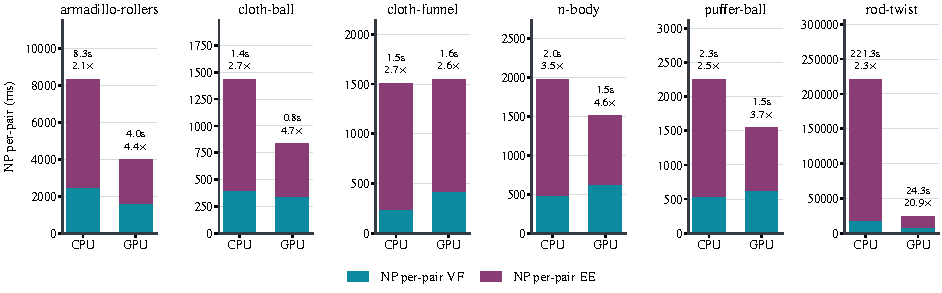
\includegraphics[width=\linewidth]{figures/reference-speedup.pdf}
  \caption{The narrow phase against TightInclusion, per scene, as whole-scene
    totals. Neither side runs a broad phase, so both are handed the same curated
    query sets and asked for one time of impact per candidate pair. Each bar is
    one processor, stacked into its vertex-face and edge-edge work, with the
    total and the speedup above it. Query counts are in \cref{tab:dataset} and
    hit agreement in \cref{tab:conservativeness}.}
  \label{fig:reference}
\end{figure}

The worst cases are a property of the problem. On cloth-funnel and rod-twist the
largest error approaches $1.0$ for the reference as well: a conservative search
has no tighter answer available on a grazing or already-touching configuration,
since the root box cannot be refined away when the contact occurs at the start
of the step.

\subsection{CPU against GPU}
\label{sec:results:proc}

\begin{table}[htbp]
  \centering
  \caption{Host against device for the same mode and the same cases. Every time is a whole-scene total in milliseconds, summed over every case of the scene. \emph{BP full} is the whole broad phase, the acceleration structure plus the queries over it; \emph{BP prep} is the structure alone and \emph{BP queries} the queries alone; \emph{NP} is the narrow phase. \emph{total} is BP full + NP, median over repeats. A ratio above one means the GPU is faster.}
  \label{tab:processor}
  \fittable{%
\begin{tabular}{lrrrrr}
    \toprule
    scene & CPU ms & GPU ms & total$\times$ & BP full$\times$ & NP$\times$ \\
    \midrule
    armadillo-rollers & 3,335 & 4,790 & 0.70x & 0.81x & 0.46x \\
    cloth-ball & 2,356 & 1,240 & 1.90x & 1.64x & 3.40x \\
    cloth-funnel & 2,073 & 3,892 & 0.53x & 0.56x & 0.41x \\
    n-body & 17,319 & 7,398 & 2.34x & 1.67x & 12.13x \\
    puffer-ball & 99,117 & 28,257 & 3.51x & 2.90x & 15.14x \\
    rod-twist & 75,502 & 37,829 & 2.00x & 2.02x & 1.97x \\
    \bottomrule
  \end{tabular}}
  \par\smallskip\footnotesize A ratio is the host median over the device median, so 2.0 means the device takes half the time. Ratios below 1.0 are the cases where the host wins and are the ones worth reading.
  \par\smallskip\footnotesize Source: \texttt{benchmark/results/sweep-gh200-bp.csv}
\end{table}


\Cref{tab:processor} reports the two processors as whole-scene totals, and the
split follows \cref{sec:parallel:why}. The broad phase is count, prefix sum and
scatter, and it runs between $0.45\times$ and $2.45\times$ of host speed. The
narrow phase is a divergent depth-first search and spans a far wider range,
$0.49\times$ to $16.51\times$: behind the host where the candidate lists are
smallest, and ahead by an order of magnitude on n-body and puffer-ball, where
billions of candidates keep every lane busy. The device's margin rests on the
narrow phase, and the broad phase decides how much of it survives.

End to end the two effects cancel to different degrees. The device wins
cloth-ball by $2.37\times$, rod-twist by $2.06\times$, n-body by $2.05\times$
and puffer-ball by $1.88\times$; the host wins armadillo-rollers at $0.95\times$
and cloth-funnel at $0.96\times$, both within five per cent of parity. On
cloth-funnel the device's broad phase is ahead at $1.29\times$ and its narrow
phase behind at $0.64\times$, so the narrow phase alone carries that scene's
gap. The two scenes the host takes are the two smallest by candidate pairs,
$25.2$ and $85.3$ million, and the device takes every scene from $175$ million
upwards. Above that the margin falls as the problem grows, cloth-ball at $175$
million pairs giving $2.37\times$ where puffer-ball at $7.33$ billion gives
$1.88\times$, so problem size indicates the processor without setting the
margin. \Cref{sec:results:scaling} varies it directly.

\Supp{} states the same comparison as a rate and per simulation step, and plots
the per-step cost through each scene. Two observations there qualify the
medians: on cloth-funnel the device is behind on $82\%$ of the frames, so its
$0.96\times$ is a standing gap and not a few expensive frames, and on rod-twist
the cost climbs steadily on both processors as the rod winds up, so the median
understates the end of the simulation.

\Cref{fig:breakdown} splits the same runs by phase: the broad phase takes $19$
to $65\%$ of the host total on every scene and $24$ to $93\%$ on the device, and
within the host's broad phase the structure it builds is the part that scales
worst with thread count (\cref{sec:results:threads}). Behind those medians,
broad-phase time is tight around its own median while narrow-phase time is
skewed by a long upper tail, the per-case form of the heavy-tailed difficulty of
\cref{tab:difficulty}; \supp{} gives the distributions. \Cref{fig:toierr} gives
the earliness distribution, one-sided by construction since every value is the
distance \emph{before} the true root at which the answer falls, with additive
CCD on the same cases beneath it.

\begin{figure}[htbp]
  \centering
  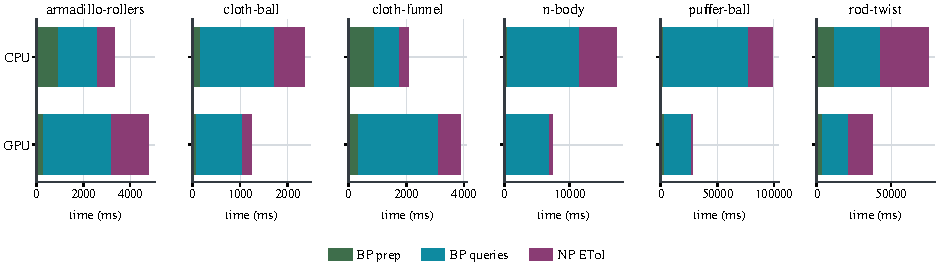
\includegraphics[width=\linewidth]{figures/runtime-breakdown.pdf}
  \caption{Whole-scene totals split into BP full and NP EToI, as a share of each
    processor's total. The BP bar is shaded into BP prep, the structure it
    builds, and BP queries over it. BP full dominates on the host, and within it
    BP prep.}
  \label{fig:breakdown}
\end{figure}

\begin{figure}[htbp]
  \centering
  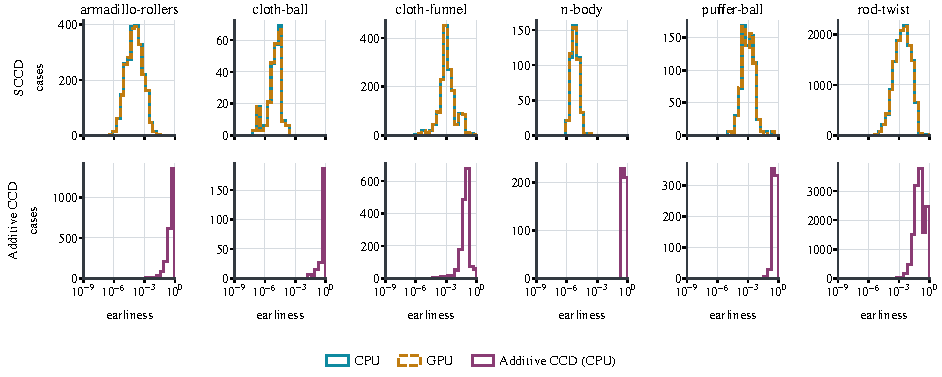
\includegraphics[width=\linewidth]{figures/earliness.pdf}
  \caption{Earliness against the exact symbolic roots, logarithmic axis, one
    value per case: the largest earliness anywhere in that case. Above, SCCD on
    both processors; below, additive CCD on the same cases, from the one
    comparison run of \cref{sec:results:others} and in the same bins. Every
    reported time of impact lies at or before its root, so both distributions
    sit on the early side of zero and nothing falls outside the axis on the late
    side. Additive CCD's
    median case sits between $1.6$ and $4.8$ decades further from the root,
    depending on the scene.}
  \label{fig:toierr}
\end{figure}

\subsection{Against other implementations}
\label{sec:results:others}

Two further implementations answer neighbouring questions, and each is compared
on the question it answers: Scalable CCD~\citep{belgrod2025toi} returns one
earliest time of impact for a simulation step, and additive
CCD~\citep{li2021codim} returns one per pair. Both are used exactly as released,
built with the same compiler flags, and run on the same node over all six scenes
and all $6{,}394$ cases, three repeats each, over identical broad-phase
candidates. \Cref{fig:competitors} summarises both comparisons per scene;
\supp{} carries the per-scene tables with their accuracy columns.

\begin{figure}[htbp]
  \centering
  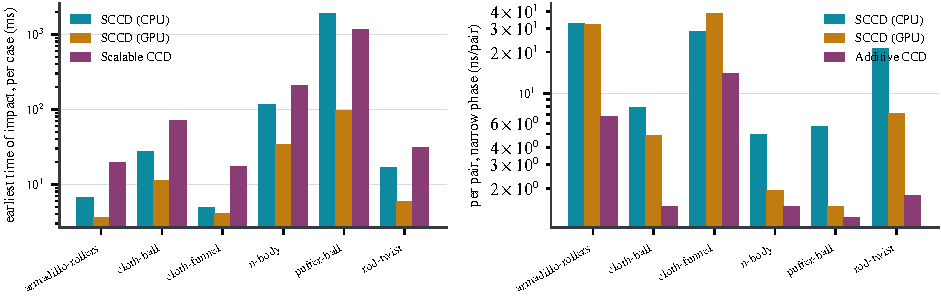
\includegraphics[width=\linewidth]{figures/competitors.pdf}
  \caption{SCCD against the two implementations that answer neighbouring
    questions, each on the question it answers. \textbf{Left}, the earliest time
    of impact for a simulation step against Scalable CCD, as the mean cost of one
    case on a logarithmic axis. \textbf{Right}, one time of impact per candidate
    pair against additive CCD, in nanoseconds per candidate.}
  \label{fig:competitors}
\end{figure}

Against Scalable CCD, SCCD on the device is ahead end to end on every scene,
from $4.23\times$ on cloth-funnel to $11.93\times$ on puffer-ball: $27.0$
against $142.9\,\mathrm{s}$ over rod-twist's $4{,}571$ cases, and $23.3$ against
$278.3\,\mathrm{s}$ over puffer-ball's $240$. Puffer-ball is also the scene on
which our host path loses outright, at $458.6\,\mathrm{s}$, since its broad
phase carries the scene on its own. The comparison is on the device throughout,
because the narrow phase of Scalable CCD is CUDA and its host side is a broad
phase with no pipeline behind it.

\Cref{fig:bpvs} compares the two broad phases step by step. Summed over the
benchmark ours costs $40.3\,\mathrm{s}$ against $312.6\,\mathrm{s}$, and the
margin is a standing one: on puffer-ball, the scene with the most candidate
pairs, it is $21.9\,\mathrm{s}$ against $226.8$. Drawing both of our strategies
separates what the implementation earns from what the choice of algorithm earns.
On n-body the two differ, our sweep being the slower broad phase there,
$7.5\,\mathrm{s}$ against Scalable CCD's $6.3$, while our cell list takes the
scene at $4.5$; on cloth-funnel the two are within $18\%$ of each other and both
far ahead, so the $5.4\times$ against Scalable CCD is attributable to the
implementation.

\begin{figure}[htbp]
  \centering
  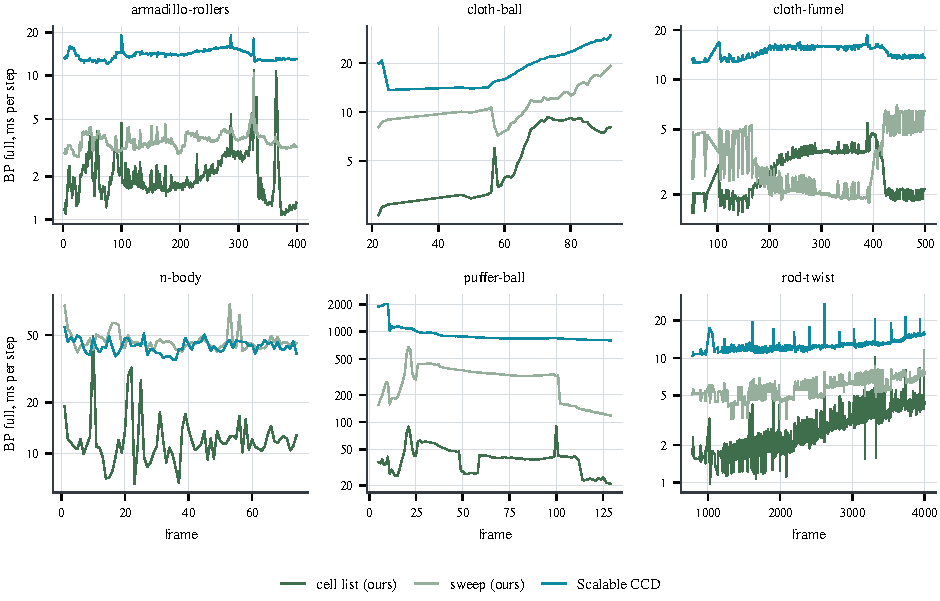
\includegraphics[width=\linewidth]{figures/broad-vs-scalable.pdf}
  \caption{Device BP full against Scalable CCD's, step by step, the
    acceleration structure and the queries over it added, in milliseconds for
    one step, both query types together. All three curves come from one
    comparison run, so they are measured in one allocation. Both of our
    strategies are drawn, since the choice between them accounts for part
    of the difference.}
  \label{fig:bpvs}
\end{figure}

Its earliness columns report a defect on three scenes and not a difference in
tightness: its answer lands after the true root on $269$ of armadillo-rollers'
$394$ contact-carrying steps, $31$ of rod-twist's $2{,}481$ and $9$ of
cloth-funnel's $363$. We traced this to a race in its subdivision buffer, whose
overflow check tests that the buffer is full and then advances the tail as two
separate operations; \supp{} gives the three observations that identify it. We
report the library as published. Where it does stay conservative it remains the
looser answer, against our device by $50.7\times$ on cloth-ball, $281\times$ on
rod-twist and $2{,}844\times$ on puffer-ball.

Additive CCD advances conservatively until contact without isolating a root, and
it is the cheaper narrow phase per candidate: by $7.1\times$ on rod-twist,
$4.9\times$ on armadillo-rollers, $2.7\times$ on cloth-funnel and $2.3\times$ on
cloth-ball, against our narrow phase on the host. The margin closes as the problem
grows, and on the two scenes carrying the most candidate pairs the two meet, at
$1.0\times$ on n-body and $1.1\times$ on puffer-ball, where billions of
candidates keep every lane of the host busy.

The cost of that speed is the answer. Its median earliness runs from
$2.3\times10^{-2}$ to $1.1\times10^{-1}$ where ours runs from
$3.0\times10^{-8}$ to $3.2\times10^{-4}$, which \cref{fig:toierr} shows as a
separation of between $1.9$ and $6.3$ decades, and its worst case gives up almost
the entire step on every scene, between $0.897$ and $0.996$. The false positives
follow: $444$ against $24$ on armadillo-rollers and $27{,}374$ against $536$ on
puffer-ball. Neither library misses a contact anywhere and neither
answers after a root, which for both follows from the construction of the method
rather than from the measurement. A solver pays for the gap with a shortened step.

\subsection{Scaling with element count}
\label{sec:results:scaling}

The refinement study reported in \supp{} refines one surface repeatedly,
quadrupling the element count at each level from $92{,}230$ to $94.4$ million
over cloth-ball frames $0$ and $1$. Both processors run the shipped broad phase,
so the one quantity it varies is the processor, and the two frames do not come
into contact, which makes the broad phase the quantity it measures.

\begin{figure}[htbp]
  \centering
  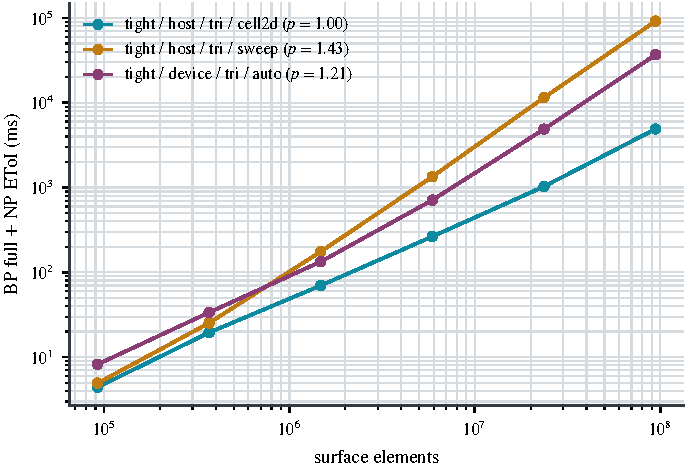
\includegraphics[width=0.62\linewidth]{figures/refine-scaling.pdf}
  \caption{Cost of one collision step against element count, log--log. Each
    series is one processor, and $p$ is the exponent fitted to the plotted
    quantity, BP full plus NP EToI.}
  \label{fig:scaling}
\end{figure}

\Cref{fig:scaling} plots both processors on logarithmic axes; they cross between
$5.90$ and $23.6$ million elements, and the device leads above that size. Taking
the whole broad phase, the host is ahead through the middle of the range by at
most $1.29\times$ ($51.6\,\mathrm{ms}$ against $66.7$ at $1.48$ million), and its
margin has already closed to $1.07\times$ at $5.90$ million ($243.7$ against
$260.7$). Past the crossing the device pulls away: $2.34\times$ at $23.6$ million
($343.5$ against $802.9$) and $2.58\times$ at $94.4$ million ($1472.5$ against
$3801.9$). The fitted exponents place the device at $0.80$ in the element count
and the host at $1.03$.

The two halves of the broad phase divide differently by processor. At $94.4$
million elements the structure costs $50.4\,\mathrm{ms}$ on the device and
$808.9$ on the host, a factor of $16.0$, while the queries over it take
$1422.2\,\mathrm{ms}$ against $2993.0$, a factor of $2.10$. The structure is
therefore $3.4\%$ of the device's broad phase and $21.3\%$ of the host's: binning
is a counting sort, the histogram is a reduction over the element count, and both
are shapes the device answers at full width. The queries carry the remainder, and
their smaller factor is what sets the device's slope.

The narrow-phase column measures a different quantity, since no root is ever
isolated on these two frames and it therefore prices the rejection test alone
over candidates that all fail it. That work is uniform, the shape a GPU handles
best: the device stays between $2.7$ and $9.2\,\mathrm{ms}$ across the six
refinements while the host climbs from $0.3$ to $130.8$, ending $14.2\times$
ahead on a column where it began $10.0\times$ behind. It is silent on the
divergent case, for which \supp{} gives narrow-phase cost against problem
size.

\subsection{Scaling with thread count}
\label{sec:results:threads}

\Cref{sec:results:scaling} varies the problem and holds the machine fixed.
Holding the problem fixed instead and varying the thread count from one to
seventy-two Grace cores separates the phases of the host pipeline
(\cref{fig:strong}).

Two of the three scale well. The overlap queries reach $32.0\times$ and the
narrow phase $40.4\times$ at seventy-two cores, which is what \cref{alg:host} is
built for: lanes are filled from a work list private to a block, blocks are
independent, and the only shared state is an atomic minimum written rarely.

Building the acceleration structure is the limit. It reaches $5.9\times$ at
thirty-two cores and goes no further, so a pass taking $8$ to $13\%$ of the
single-core time takes $38$ to $48\%$ of it at seventy-two and holds the whole
pipeline to between $13.2\times$ and $24.0\times$. Three passes over every box
account for the plateau, all of them reductions or histograms: the
centre-variance reduction that picks the two grid axes, the extent and mean
reduction that sizes the grid, and the counting histogram that fills it. What
remains once those are parallel is a fixed cost per call rather than a share of
the work, which is why further cores cannot recover it --- between sixty-four and
seventy-two cores every curve is flat, so none of the figures quoted here depends
on which of the two counts it is read at.

\begin{figure}[htbp]
  \centering
  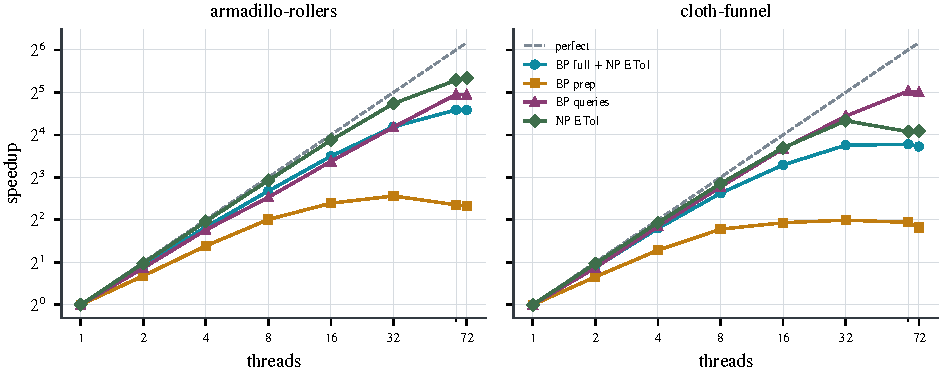
\includegraphics[width=\linewidth]{figures/strong-scaling.pdf}
  \caption{Strong scaling of the host pipeline by phase, as whole-scene totals
    against the perfect line. The narrow phase tracks it closely; the structure
    the broad phase builds leaves it early and plateaus around thirty-two cores.}
  \label{fig:strong}
\end{figure}
